\documentclass{beamer}
\usetheme{metropolis}
%\usecolortheme{owl}
\usepackage{url}
\usepackage{underscore}
\usepackage{xcolor}
\definecolor{dark}{HTML}{23373b}
\definecolor{bright}{HTML}{EB811B}
\definecolor{white}{HTML}{FFFFFF}

% Tikz
\usepackage{tikz}
\usetikzlibrary{fit,backgrounds}
\tikzset{
    vertex/.style = {
      circle,
      fill = black,
      outer sep = 2pt,
      inner sep = 1pt,
    },
    task/.style = {
      rounded corners,
      fill=dark,
      text=white,
      text width=2cm,
      align=center
    },
    input/.style = {
    },
    stepp/.style = {
      fill=bright!80,
      rounded corners
    }
}
% Beamer
\title{CDS}
\subtitle{Video Submission (Backend)}
\date{January 27, 2017}
\author{Orestis Melkonian}
\institute{CERN, IT-CDA-DR}

% Box macro
\newcommand{\contrib}[1]{
  \vfill
  \begin{alertblock}{Invenio Framework}
    #1
  \end{alertblock}
}

\begin{document}  
  \metroset{block=fill, background=dark}
  \setbeamercolor{block body}{fg=white}
	\maketitle
	
	\begin{frame}{Overview}
    \begin{itemize}
      \item{Currently, submission is handled externally}
      \item{Moved towards an in-house solution}
      \item{Single page with multiple deposits (i.e. \alert{Project})}
      \item{Specific workflow in the background for each project}
    \end{itemize}
	\end{frame}
  
	\section{The AV Workflow}
  \begin{frame}{Workflow}
    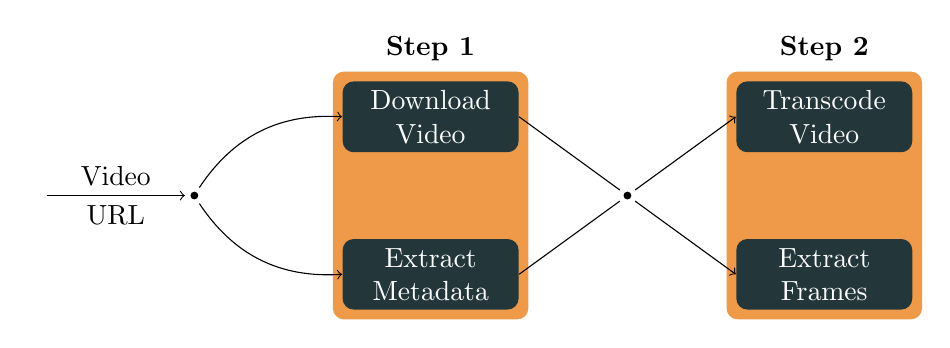
\begin{tikzpicture}
      \node         (I) at (-2, 0) {};
      \node[vertex] (V) at (0,  0) {};
      \node[task]   (D) at (3,  1) {Download Video};
      \node[task]   (M) at (3, -1) {Extract Metadata};
      \node[vertex] (J) at (5.5,  0) {};
      \node[task]   (T) at (8,  1) {Transcode Video};
      \node[task]   (F) at (8, -1) {Extract Frames};
 
      \draw[->] (I) -- node[above] {Video} node[below] {URL} (V);
      \draw[->] (V) to[bend left] (D.west);
      \draw[->] (V) to[bend right] (M.west);
      \draw[-] (D.east) -- (J);
      \draw[-] (M.east) -- (J);
      \draw[->] (J) -- (T.west);
      \draw[->] (J) -- (F.west);
      
      \begin{scope}[on background layer]
        \node[stepp, fit=(D) (M), label=above:\bf{Step 1}] {};
        \node[stepp, fit=(T) (F), label=above:\bf{Step 2}] {};
      \end{scope}
    \end{tikzpicture}
	\end{frame}
  
	\section{Invenio Video Toolkit \newline \it{(Name in Progress)}}
  \begin{frame}{Video Processing API}
    	\begin{itemize}
		  \item{Transcoding}
		  \begin{itemize}
		    \item{\emph{start_encoding}}
		    \item{\emph{stop_encoding}}
		    \item{\emph{get_encoding_status}}
    	  \end{itemize}
		  \item{\emph{extract_metadata}}
		  \item{\emph{extract_frames}}
		  \item{Configured as import strings, in order to allow \alert{multiple backends}}
	  \end{itemize}

	  \contrib{
	    This work will lead to the creation of a general video toolkit for \emph{Invenio}, which will include the wrappers for \alert{FFmpeg} and \alert{Sorenson}.
	  }
	\end{frame}

	\section{Server-sent Events (SSE)}
	\begin{frame}{Motivation}
	    	\begin{itemize}
    	  \item{A way to update the UI \alert{asynchronously}}
		  \item{Better alternative to polling}
    		\begin{itemize}
    		  \item{Responsive}
    		  \item{Data-driven}
	  	  \end{itemize}
	  \end{itemize}
	\end{frame}
	
	\begin{frame}{Usage}
    	\begin{itemize}
    		\item{Channel per project}
    		\item{Type per task}
    		\item{Access rights}
	  \end{itemize}
	  
	  \contrib{
		  Basic SSE functionality and integration with \emph{InvenioDeposit} is implemented on the new \emph{Invenio} module \alert{InvenioSSE}.
		}
	\end{frame}

	\section{Tasks}
	\begin{frame}{Webhooks}
    	  Extended REST API of \emph{InvenioWebhooks}
    	  \begin{itemize}
    	    \item{\url{hooks/receivers/<rid>/events/<eid>/tasks/<tid>}}
    	    \item{Allows fine-grained control of individual tasks on a single event}
    	    \item{\alert{DELETE} $\rightarrow$ cancel}
    	    \item{\alert{PUT} $\rightarrow$ restart}
      \end{itemize}
	\end{frame}
	\begin{frame}{SSE Tasks}
      	Extended \emph{Celery's} task base class for SSE integration. \\
      	\vfill
      	Overloaded some task methods to additionally send appropriate SSE:
  	    \begin{itemize}
    	    \item{\emph{update_state}}
    	    \item{\emph{on_success}}
    	    \item{\emph{on_failure}}
    	    \item{\emph{on_revoke}}
  	    \end{itemize}
	\end{frame}
	
	\begin{frame}{Cancelable \& Undo-able Tasks}
	  Extended \emph{Celery's} task base class for safe cancel/undo. \\
	  \begin{itemize}
	    \item{Every task must implement the \alert{clean} method}, which should undo any side-effects from its execution.
	    \item{Imposes explicit resource management}
	  \end{itemize}
	\end{frame}

  \section{Miscellaneous}
  	\begin{frame}{File Tags}
    	\begin{itemize}
    	  \item{Store video's metadata}
    	  \item{File relationships (e.g. \emph{master file})}
    	  \item{File types (e.g. \emph{video}, \emph{frame})}
	  \end{itemize}

	  \contrib{
		  Tags were added as an extra feature in \alert{InvenioFilesRest}.
    	}
	\end{frame}

  	\begin{frame}{Data Model}
    	\begin{itemize}
    	  \item{Defined new schemas for \alert{Project} and \alert{Video}}
   	  \item{Inspired by widely-used solutions (e.g. schema.org)}
	  \end{itemize}
	\end{frame}
	
	\begin{frame}{Report Number Generation}
	  \begin{itemize}	  
    	  \item{\alert{Project}}
      	\begin{itemize}
      	  \item{Report number is automatically generated on publish}
      	  \item{Uses the record's metadata (i.e. \emph{category, type, year})}
    	  \end{itemize}
    	  \item{\alert{Video}}
      	\begin{itemize}
      	  \item{Utilizes the hierarchical sequences}
      	  \item{Child sequence of \emph{Project}}
    	  \end{itemize}
  	  \end{itemize}

  	   \contrib{
		  Complete rewrite of \alert{InvenioSequenceGenerator}.
		}    	
	\end{frame}

\end{document}